Skalibrowany w ten sposób model integruje ze sobą strukturę czasową komponentów spreadu oraz ich współzależności. Całą strukturę można teraz odwrócić, żeby otrzymać model symulujący ścieżki komponentów spreadu, a finalnie samego spreadu. Wykonujemy w tym celu następujący algorytm:
\begin{enumerate}
	\item Z dopasowanej struktury Vine Copula losujemy 3 ciągi jednostajnych obserwacji.
	\begin{itemize}
		\item Efektem są ciągi $IID\sim\mathcal{U}(0, 1)$, o strukturze zależności zadanej przez Vine Copula.
	\end{itemize}
	\item Używamy jednostajnych ciągów oraz wyestymowanych wcześniej empirycznych dystrybuant do metody odwrotnej dystrybuanty.
	\begin{itemize}
		\item Efektem są wysymulowane rezidua modelu GARCH(2, 3) o odpowiedniej strukturze zależności.
	\end{itemize}
	\item Używamy wysymulowanych reziduów, żeby dokonać predykcji logzwrotów według modeli ARIMA-GARCH(2, 3) dla każdego aktywa. 
	\begin{itemize}
		\item Efektem są wysymulowane logzwroty dla każdego aktywa, o odpowiedniej strukturze zależności.
	\end{itemize}
	\item Używamy wysymulowanych logzwrotów razem z ostatnią dostępną wartością ze zbioru danych, żeby dokonać predykcji trajektorii dla każdego aktywa. 
	\begin{itemize}
		\item Efektem są wysymulowane trajektorie dla każdego aktywa, o odpowiedniej strukturze zależności.
	\end{itemize}
	\item Używamy wysymulowanych trajektorii aktywów żeby obliczyć trajektorię soybean crush spreadu.
	
\end{enumerate}
\begin{figure}[h]
	\centering
	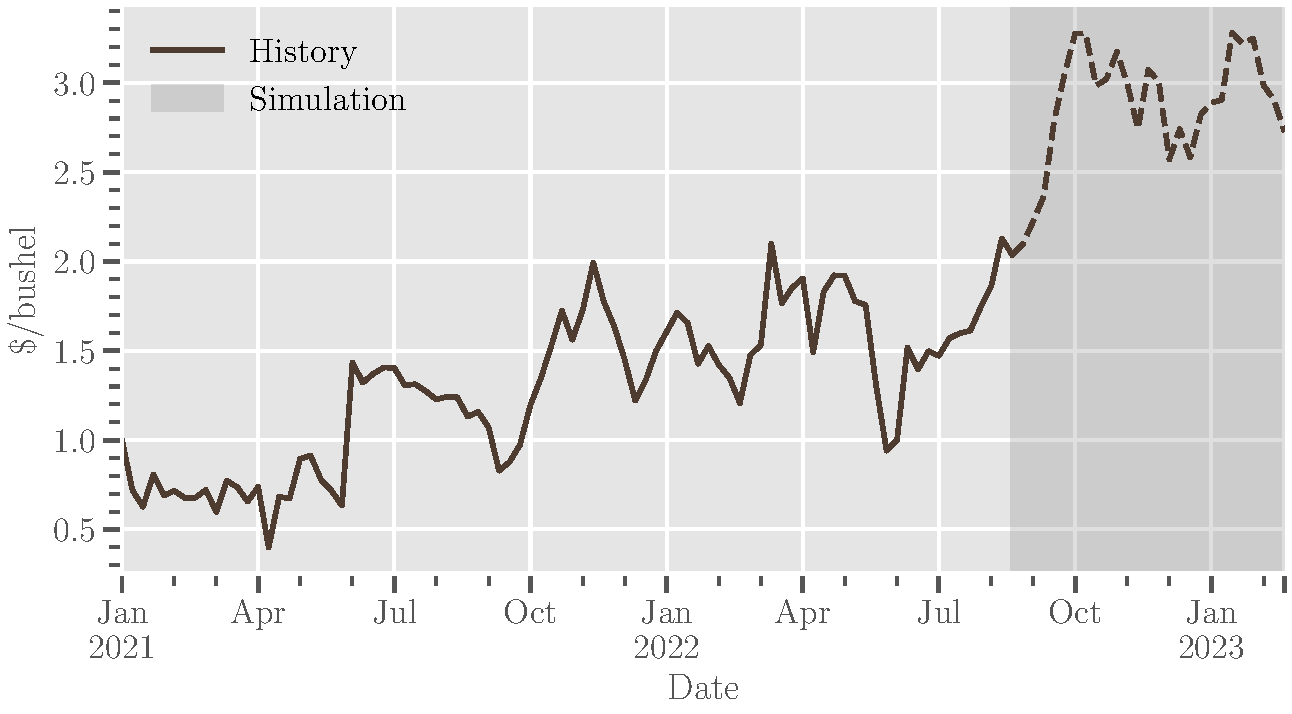
\includegraphics[width=0.8\linewidth]{04_SimulationSpread}
	\caption{\textbf{Symulacja trajektorii (1/2).} Przykładowa $6$-miesięczna symulacja crush spreadu, zgodnie z dopasowanym modelem.\label{fig:simulation_spread}}
\end{figure}

Rysunek \ref{fig:simulation_spread} przedstawia przykładowy wynik takiej symulacji dla crush spreadu. Widzimy, że wysymulowana trajektoria jest wiarygodna biorąc pod uwagę kontekst historii szeregu czasowego (tj. w sensie poziomu, oscylacji, czy dynamiki).\\

Możemy użyć metody Monte Carlo w celu otrzymania nie pojedynczej trajektorii, ale wielu możliwych realizacji, a następnie użyć tych symulacji do wyceny instrumentów pochodnych na spread. Zaprezentujemy ideę na przykładzie europejskich opcji na spread, o parametrach:
\begin{itemize}
	\item Instrument pierwotny: soybean crush spread $s(t)$
	\item Termin wygaśnięcia: $T = 27$ tygodni
	\item Ceny wykonania: od $0.5\times K$ do $1.5\times K$, gdzie $ATM = K \approx\$2$/buszel
	\item Money-market rate: $r = 5\%$
\end{itemize}

Podobnie jak w \cite{Bernard_Pricing_Multivariate_Options_with_copulae}, czy  \cite{Herath_Copula_Crack_Spread} przeprowadziliśmy powtórzenia Monte Carlo, w trakcie których dla każdej ścieżki obliczona została wypłata opcji kupna i sprzedaży, a następnie wyniki zostały uśrednione i zdyskontowane. W ten sposób otrzymujemy finalną cenę opcji w mierze rzeczywistej. 
Rysunek \ref{fig:simulation_monte_carlo} prezentuje wynik symulacji trajektorii spreadu w postaci rozkładu wysymulowanych wartości dla każdego punktu czasowego (każdego tygodnia), natomiast rysunek \ref{fig:payoffs_distribution} pokazuje rozkład spreadu w momencie wygaśnięcia opcji, wraz z rozkładem wypłat opcji call i put. Średnia wypłata, zdyskontowana do chwili $T=0$ daje cenę opcji - co prezentujemy dla różnych cen wykonania w tabeli \ref{tab:option_prices}.\\
\begin{figure}[h]
	\centering
	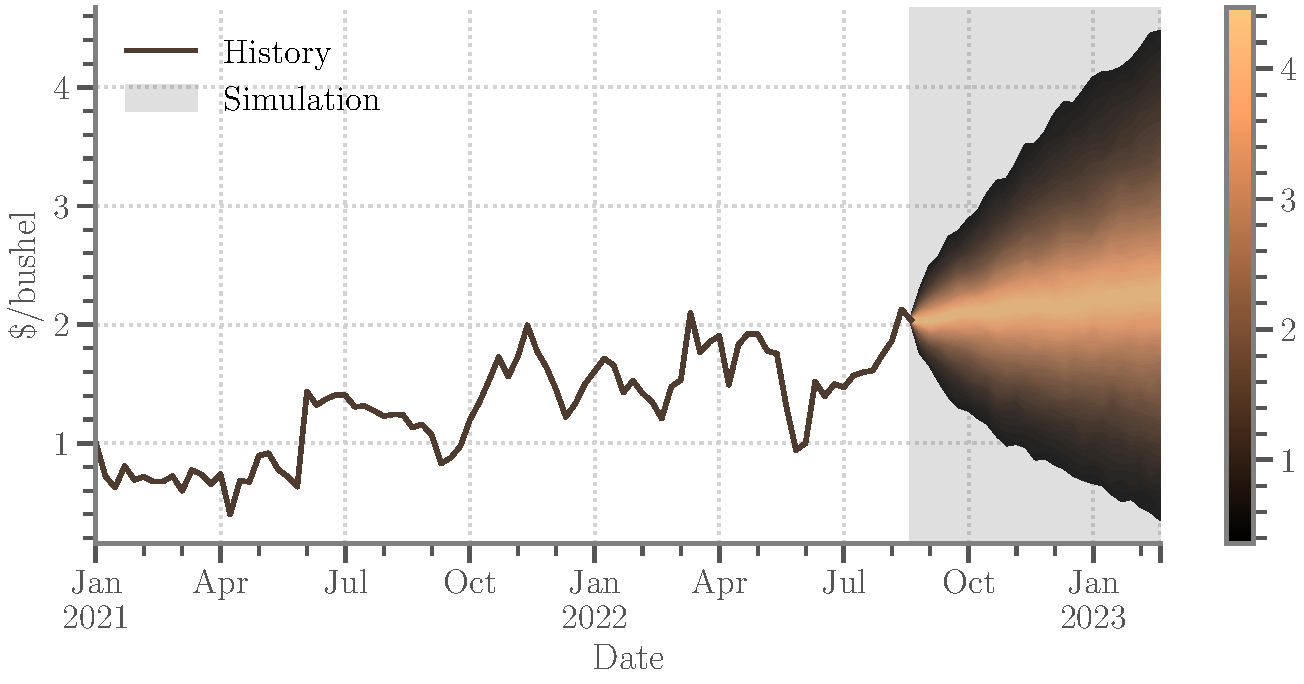
\includegraphics[width=0.9\linewidth]{04_CrushSpread_pred}
	\caption{\textbf{Symulacja trajektorii (2/2).} Rozkład symulacji Monte Carlo $6$-miesięcznych trajektorii crush spreadu. \label{fig:simulation_monte_carlo}}
\end{figure}


\begin{figure}[h]
	\centering
	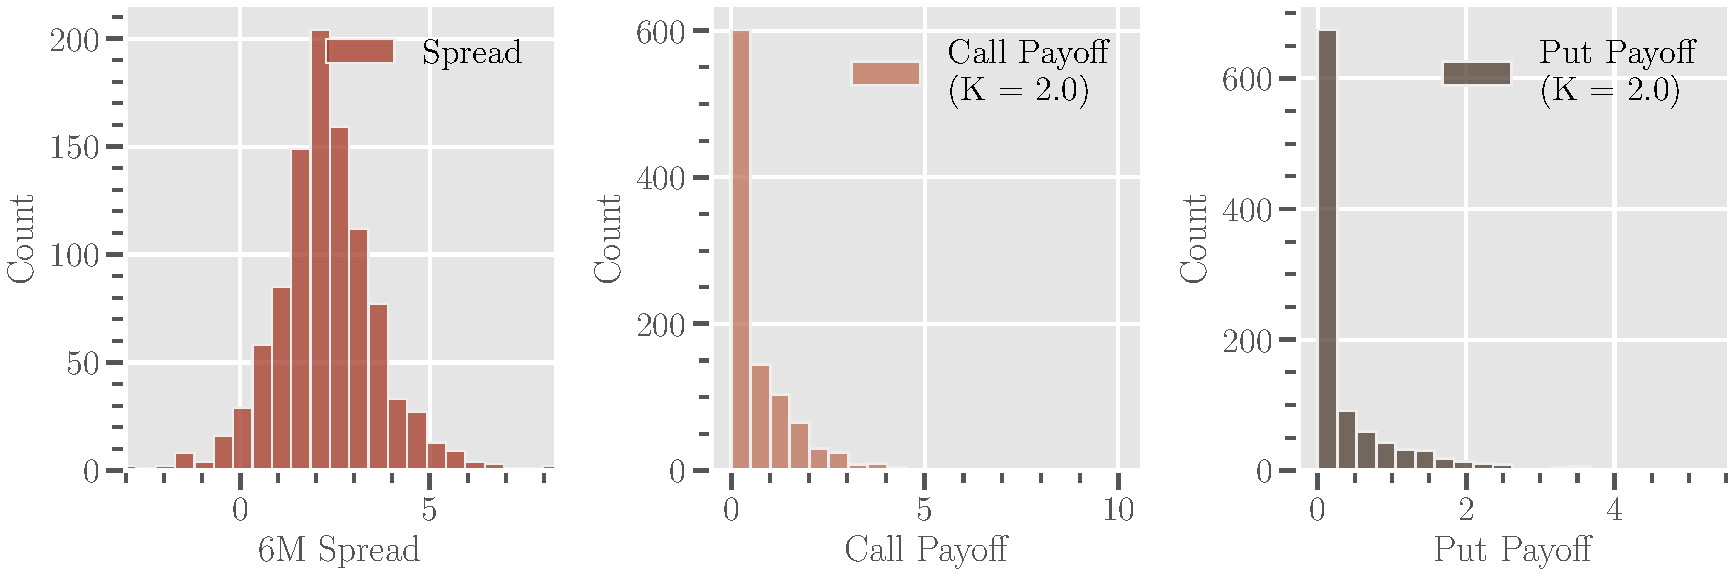
\includegraphics[width=\linewidth]{04_PayoffsDistribution}
	\caption{\textbf{Moment wykonania opcji.} Histogram wysymulowanych spreadów (lewy panel), oraz histogramy wypłat z opcji: call (środkowy panel) i put (prawy panel), przy cenie wykonania $K=2.0$. \label{fig:payoffs_distribution}}
\end{figure}


\begin{table}
	\centering
	\csvreader[
	tabular=r|cccc,
	table head=\toprule  & \multicolumn{2}{c}{\bfseries{Call}} & \multicolumn{2}{c}{\bfseries{Put}} \\ 
\bfseries{Strike} & \bfseries{Price} & \bfseries{Std. Err.} & \bfseries{Price} & \bfseries{Std. Err.}\\\midrule,
	table foot = \bottomrule
	]{
		Tables/OptionPrices.csv
	}{}{\csvlinetotablerow}
	
	\caption{\textbf{Ceny europejskich opcji.} Ceny opcji europejskich kupna i sprzedaży w modelu symulacyjnym ARIMA-GARCH-VineCopula, razem z ich błędami standardowymi. Wyniki otrzymane metodą Monte Carlo dla $1000$ powtórzeń. \label{tab:option_prices}}
\end{table}

\FloatBarrier
Na koniec, w celu zilustrowania istotnego wpływu zastosowania Vine Copula, rozważyliśmy sytuację w której model zostałby uproszczony i zamiast struktury Vine do modelowania zależności użytoby najprostszego modelu GMV (gaussian multivariate copula). Rysunek \ref{fig:model_comparison} prezentuje porównanie rozkładu trajektorii spreadu między tymi dwoma modelami. Zaobserwować można, że użycie wielowymiarowej kopuły gaussowskiej skutkuje uchwyceniem ciężkoogonowego charakteru spreadu, oraz że kwantyle dla większości rzędów przebiegają blisko kwantyli powstałych z modelu Vine Copula. Jednak istnieje istotna różnica, widoczna w kwantylach ekstremalnych rzędów, jak $0.01$ czy $0.99$ które udowadniają, że model Vine Copula uchwyca jeszcze cięższe ogony logzwrotów spreadu w stosunku do modelu GMV.
	
\begin{figure}[h]
	\centering
	\begin{minipage}{\linewidth}
	\centering
	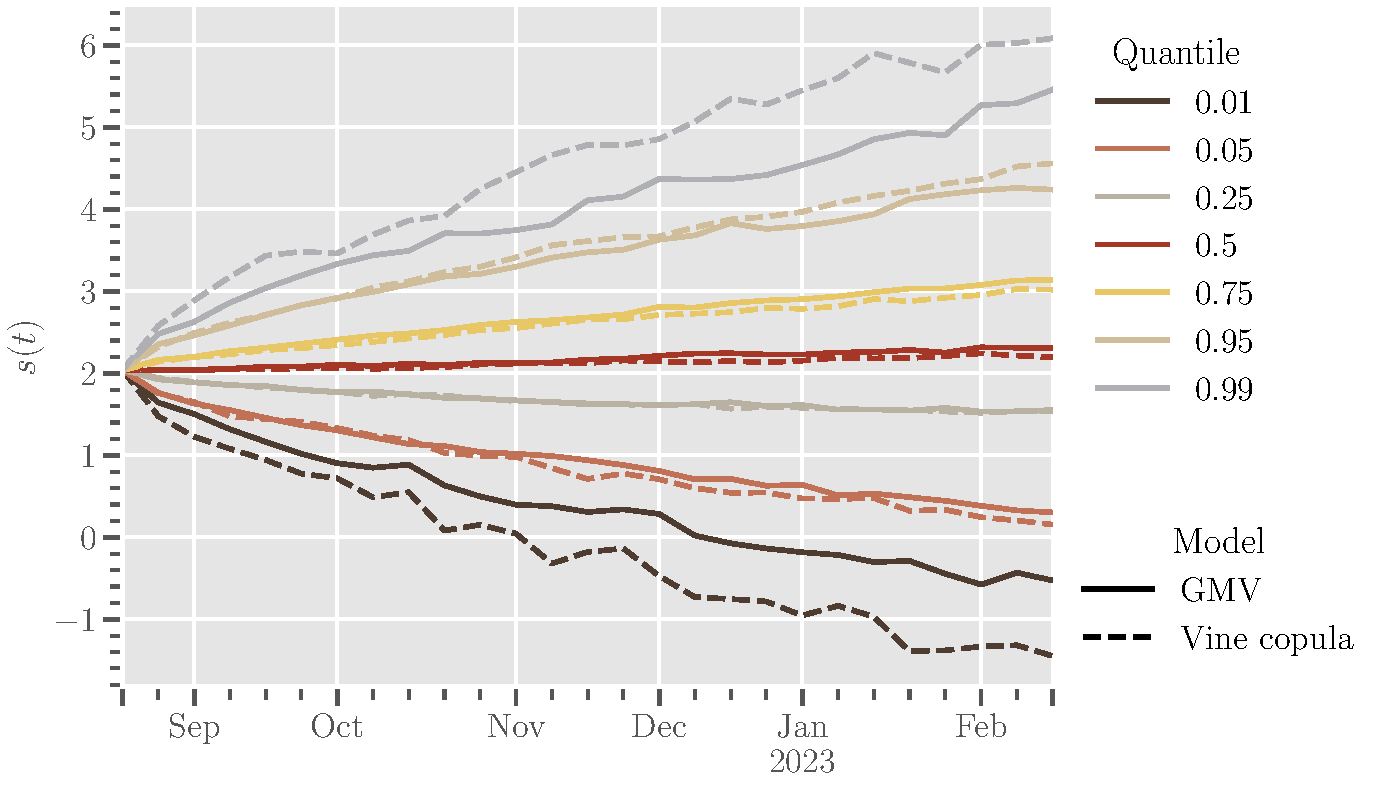
\includegraphics[width=0.8\linewidth]{04_MVG_Vine_quantile_comparison}
	\end{minipage}

	\begin{minipage}{\linewidth}
	\centering
	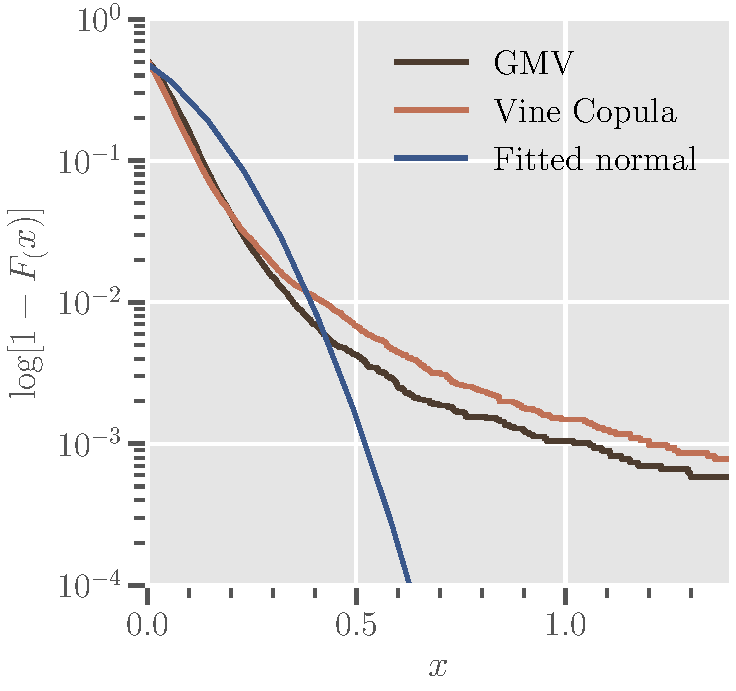
\includegraphics[width=0.5\linewidth]{04_TailComparison}
	\end{minipage}

	\caption{\textbf{Porównanie modeli.} Kwantyle trajektorii wysymulowanych spreadów przy pomocy wielowymiarowej kopuły normalnej (GMV), oraz Vine Copula (górny panel). Porównanie ciężkości ogonów logzwrotów spreadu (dolny panel).\label{fig:model_comparison}}

\end{figure}
